% fig2-protocol.tex
% Experimental Protocol: Wild-type -> Interventions -> Comparison
\documentclass[tikz,border=9pt]{standalone}

% common-styles.tex
% Shared TikZ styles for wonton-proof paper figures

\usepackage{silence}
\WarningFilter{latex}{Missing character} 
\tracinglostchars=0 % Suppress engine-level "Missing character" warnings

\usepackage{fontspec}
\usepackage{unicode-math}

% Use filenames for reliability with Tectonic
\setmainfont{LibertinusSerif-Regular.otf}[
    BoldFont=LibertinusSerif-Bold.otf,
    ItalicFont=LibertinusSerif-Italic.otf,
    BoldItalicFont=LibertinusSerif-BoldItalic.otf
]
\setsansfont{LibertinusSans-Regular.otf}[
    BoldFont=LibertinusSans-Bold.otf,
    ItalicFont=LibertinusSans-Italic.otf
]
\setmonofont{LibertinusMono-Regular.otf}

% Try a more standard math font if LibertinusMath is causing nullfont issues
\setmathfont{LibertinusMath-Regular.otf}
% \setmathfont{latinmodern-math.otf}[range=digits] 

\usepackage{amsmath}
\usepackage{tikz}
\usepackage{forest}

\usetikzlibrary{
    arrows.meta,
    calc,
    decorations.pathreplacing,
    fit,
    positioning,
    shapes.geometric,
    shapes.misc,
    backgrounds,
    shadows.blur,
    fadings
}

% Color palette (muted, print-friendly)
\definecolor{ink}{RGB}{45,45,52}
\definecolor{muted}{RGB}{115,115,125}
\definecolor{highlight}{RGB}{198,120,44}
\definecolor{accentblue}{RGB}{86,130,178}
\definecolor{accentgreen}{RGB}{84,156,132}
\definecolor{blocked}{RGB}{140,75,75}
\definecolor{goalnode}{RGB}{255,255,255}
\definecolor{terminal}{RGB}{238,239,244}
\definecolor{deadnode}{RGB}{248,245,245}
\definecolor{flowbox}{RGB}{250,250,252}
\definecolor{basin1}{RGB}{224,234,248}
\definecolor{basin2}{RGB}{246,232,221}
\definecolor{basin3}{RGB}{228,242,234}
\definecolor{heatbase}{RGB}{86,130,178}

\tikzset{
    line cap=round,
    line join=round,
    pop/.style={
        blur shadow={shadow blur steps=5, shadow blur extra rounding=1.3pt}
    },
    base node/.style={
        rounded rectangle,
        draw=ink,
        line width=0.6pt,
        fill=goalnode,
        text=ink,
        minimum width=2.2cm,
        minimum height=0.7cm,
        align=center,
        pop
    },
    goal/.style={base node, fill=goalnode},
    terminal/.style={base node, fill=terminal, line width=0.9pt},
    dead/.style={base node, fill=deadnode, dashed},
    flowbox/.style={
        rectangle,
        draw=muted,
        rounded corners=3pt,
        fill=flowbox,
        minimum width=1.8cm,
        minimum height=0.6cm,
        align=center,
        font=\normalfont\small,
        text=ink,
        pop
    },
    decision/.style={
        diamond,
        draw=muted,
        fill=flowbox,
        aspect=2.4,
        font=\normalfont\small,
        inner sep=1pt,
        text=ink
    },
    protocolbox/.style={
        rectangle,
        draw=muted,
        rounded corners=4pt,
        fill=flowbox,
        minimum width=2cm,
        minimum height=0.8cm,
        font=\normalfont\small,
        align=center,
        text=ink
    },
    tactic/.style={
        ->,
        >=Stealth,
        draw=muted,
        line width=0.75pt
    },
    tacticlight/.style={
        ->,
        >=Stealth,
        draw=muted!45,
        dashed,
        line width=0.6pt
    },
    backprop/.style={
        ->,
        >=Stealth,
        draw=muted!70,
        dashed,
        line width=0.6pt
    },
    selected/.style={
        tactic,
        draw=highlight,
        line width=1.4pt
    },
    divergetactic/.style={
        tactic,
        draw=highlight,
        line width=1.4pt
    },
    divergenode/.style={
        base node,
        draw=highlight,
        line width=1.0pt
    },
    divergeblock/.style={
        blockedtactic,
        line width=1.2pt
    },
    blockedtactic/.style={
        tactic,
        draw=blocked,
        densely dashed
    },
    flowarrow/.style={
        ->,
        >=Stealth,
        draw=muted,
        line width=0.75pt
    },
    crosslink/.style={
        -,
        draw=muted!70,
        dotted,
        line width=0.6pt
    },
    annot/.style={
        font=\normalfont\footnotesize,
        text=muted
    },
    visit/.style={
        annot,
        font=\normalfont\scriptsize
    },
    annotbg/.style={
        annot,
        fill=white,
        inner sep=1.5pt
    },
    tacticlabel/.style={
        annot,
        font=\ttfamily\footnotesize,
        text=muted
    },
    formula/.style={
        font=\normalfont\footnotesize,
        draw=muted,
        rounded corners=2pt,
        fill=white,
        inner sep=3pt
    },
    paneltitle/.style={
        font=\normalfont\bfseries,
        text=ink
    },
    trajectory/.style={
        ->,
        draw=muted!70,
        line width=0.6pt
    }
}


\begin{document}
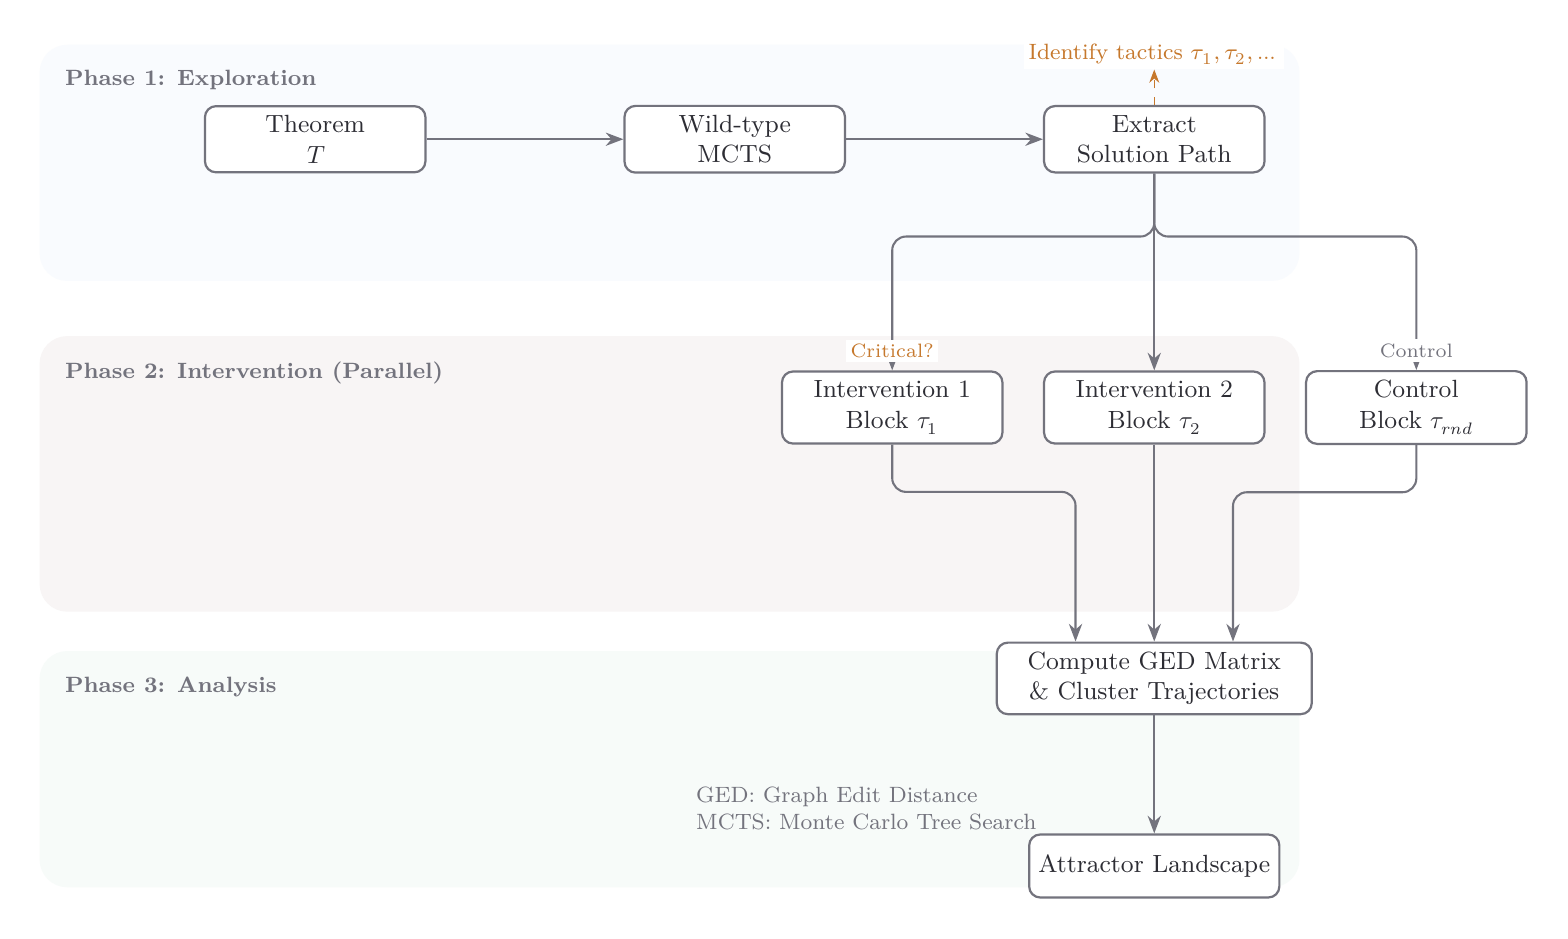
\begin{tikzpicture}[
    node distance=1.5cm and 2.5cm,
    every node/.style={font=\small},
    show background rectangle,
    background rectangle/.style={fill=white}
]

\tikzset{
    stage/.style={protocolbox, minimum width=2.8cm, fill=white, draw=muted, line width=0.8pt},
    phaselabel/.style={font=\bfseries\footnotesize, text=muted, align=center, anchor=north west}
}

% --- Background Zones ---
% Drawn first to sit behind everything
\begin{scope}
    % Phase 1: Exploration (Top)
    \fill[basin1!20, rounded corners=10pt] (-3.0, 1.2) rectangle (13.0, -1.8);
    \node[phaselabel] at (-2.8, 1.0) {Phase 1: Exploration};

    % Phase 2: Intervention (Middle)
    \fill[deadnode!100, rounded corners=10pt] (-3.0, -2.5) rectangle (13.0, -6.0);
    \node[phaselabel] at (-2.8, -2.7) {Phase 2: Intervention (Parallel)};

    % Phase 3: Analysis (Bottom)
    \fill[basin3!30, rounded corners=10pt] (-3.0, -6.5) rectangle (13.0, -9.5);
    \node[phaselabel] at (-2.8, -6.7) {Phase 3: Analysis};
\end{scope}


% --- Phase 1: Exploration ---
\node[stage] (theorem) at (0.5, 0) {Theorem\\$T$};
\node[stage, right=of theorem] (wildtype) {Wild-type\\MCTS};
\node[stage, right=of wildtype] (extract) {Extract\\Solution Path};

\draw[flowarrow] (theorem) -- (wildtype);
\draw[flowarrow] (wildtype) -- (extract);

% Tactic extraction annotation
\draw[dashed, draw=highlight, ->, >=Stealth] (extract.north) -- ++(0, 0.45)
    node[above, annotbg, text=highlight] {Identify tactics $\tau_1, \tau_2, \dots$};


% --- Phase 2: Intervention ---
% Fan-out point
\coordinate[below=1.5cm of extract] (fanout_center);

% Nodes
\node[stage, below=2.5cm of extract] (int2) {Intervention 2\\Block $\tau_2$};
\node[stage, left=0.5cm of int2] (int1) {Intervention 1\\Block $\tau_1$};
\node[stage, right=0.5cm of int2] (control) {Control\\Block $\tau_{rnd}$};

% Arrows from Phase 1
\draw[flowarrow, rounded corners=5pt] (extract.south) -- ++(0,-0.8) -| (int1.north);
\draw[flowarrow] (extract.south) -- (int2.north);
\draw[flowarrow, rounded corners=5pt] (extract.south) -- ++(0,-0.8) -| (control.north);

% Annotations
\node[annotbg, above=0.1cm of int1, text=highlight, font=\scriptsize] {Critical?};
\node[annotbg, above=0.1cm of control, text=muted, font=\scriptsize] {Control};


% --- Phase 3: Analysis ---
\node[stage, below=2.5cm of int2, minimum width=4cm] (compare) {Compute GED Matrix\\\& Cluster Trajectories};
\node[stage, below=of compare] (output) {Attractor Landscape};

% Convergence arrows
\draw[flowarrow, rounded corners=5pt] (int1.south) -- ++(0,-0.6) -| ([xshift=-1.0cm]compare.north);
\draw[flowarrow] (int2.south) -- (compare.north);
\draw[flowarrow, rounded corners=5pt] (control.south) -- ++(0,-0.6) -| ([xshift=1.0cm]compare.north);

\draw[flowarrow] (compare) -- (output);

% --- Legend / Key ---
\begin{scope}[shift={(7.5, -8.5)}]
    \node[annot, align=left] {GED: Graph Edit Distance\\MCTS: Monte Carlo Tree Search};
\end{scope}

\end{tikzpicture}
\end{document}
